\chapter{Introduction}

Circumstellar disks of gas and dust, left over from the processes of stellar formation, are cosmic nurseries for the growth of planets. In these young stellar systems, bodies ranging from small and rocky to massive and gaseous coalesce as gravitational, chemical, and viscous evolution transform gas-rich protoplanetary disks into tenuous, nearly gas-free debris disks over millions of years. While the direct detection of planets during this time is effectively impossible with our current technology, observations of rotational transitions of gas species, scattered light from micron-sized dust grains, and thermal emission from micron to millimeter-sized grains provide an indispensable tracer of the processes that shape these disks. Because the genesis of planets is directly tied to the morphology of the gas and dust, studying the anatomy of a variety of young disks is essential to understanding how worlds such as our own formed. 49 Ceti, at an estimated age of 40 million years, is just one puzzle piece of many, but its gas-rich debris disk provides important clues to deciphering the final stages of disk evolution. 

%49 Ceti is in the process of transitioning from a gas-rich disk to a tenuous, nearly gas-free debris disk, which makes it the perfect target to probe the processes by which the gas and dust dissipate.  

%Because the genesis of planets is directly tied to the morphology of the gas and dust and their development over time, observing the anatomy of nearby disks is helping us piece together the means by which planets form.  

%Characterizing the transitional phase from young, gas-rich protoplanetary disks to older, tenuous, and nearly gas-free debris disks is imperative for understanding how these planetary systems form. 

%Gas giants, such as Jupiter and Saturn, are thought to form from runaway accretion of gas onto a rocky core. However, in the 10 million years it takes the rocky core to form, most primordial gas has already disappeared. 
%Using CO as the tracer, observations have shown that the bulk of primordial gas dissipates within $\sim$ 10Myr, with less than a Jupiter mass generally remaining after only a few million years \citep{Zuck95}. Th
%and because we assume that the evolution of the gas is closely tied to that of the dust, 

%\section{Planet Formation Processes Dispersal of Gas and Dust}
\section{Planet Formation and The Evolution of Protoplanetary Disks to Debris Disks}

The collapse of giant clouds of molecular hydrogen leads directly to the formation of stars and their accompanying protoplanetary disks. As such, the mass of such a disk, which is generally on order 0.5$\%$ that of the star \citep{Andr13}, is dominated by primordial H$_{2}$. Although the dust contributes significantly less mass, a key characteristic is that it is optically thick in protoplanetary disks, but optically thin in debris disks \citep{Wyat14}. Surveys have found the median lifetime of dust disks is only a Myr \citep{Mama09} and that the bulk of primordial gas dissipates within 10\,Myr \citep{Zuck95}, putting a critical cutoff on the planet formation timeline for both rocky and gaseous planets. The ever-growing wealth of planets discovered around stars of all spectral types suggest that planetary systems are a common endpoint for the evolution of circumstellar material \citep{Howa13}. Thus, planet formation theories must show that the majority of disks can form gas planets within a few Myr, or that substantial amounts of gas persist beyond the dissipation of the optically thick dust disk. Recent statistical analyses suggest that at least $\sim$ 17$\%$ of stars host a Jupiter-mass planet (0.3-10M$_{Jup}$) and $\sim$ 52$\%$ have a Neptune-mass planet (10-30M$_{\oplus}$) \citep{Cass12}. 

The most widely accepted model of giant planet formation is that of core-accretion, in which a rocky core must coalesce before runaway accretion of gas can begin. The timescale of gas planet formation is determined almost exclusively by the amount of time it takes this core to form, which in turn is extremely sensitive to the initial surface density of the planetary nebula \citep{Poll86,Poll96}. Models by \cite{Alib05} suggest that for a disk with an initial mass on the order of the solar system's primordial nebula, core formation takes $\sim$ 1\,Myr, but those of \cite{Inab03} hint that this process takes closer to a few Myr. These timescales are right on the border of the lifetime of disks suggested observationally by \citeauthor{Mama09} and \citeauthor{Zuck95}. Because the subtleties of how core-accretion works are still uncertain, analyzing circumstellar material throughout its evolution is important for constraining modeling assumptions. 

The timeline for planet formation coincides with significant changes in the large scale structure of the disk. Characterized by the clearing of an inner hole, these ``transition disks" are readily detectible by the dearth of near-IR emission in their spectral energy distributions (SEDs), as there are few hot grains emitting at these short wavelengths \citep{Stro89}. The gravitational influence of planets and photoevaporation are both feasible means for this inside-out clearing, and the reality probably includes some combination of these processes \citep{Wyat14}. Much of the protoplanetary material is locked up in larger bodies or disappears due to photoevaporation or accretion in this time. However, small and observable grains, as well as some gas species, can be replenished through collisions in ``debris" processes. 

\begin{figure}
\centering
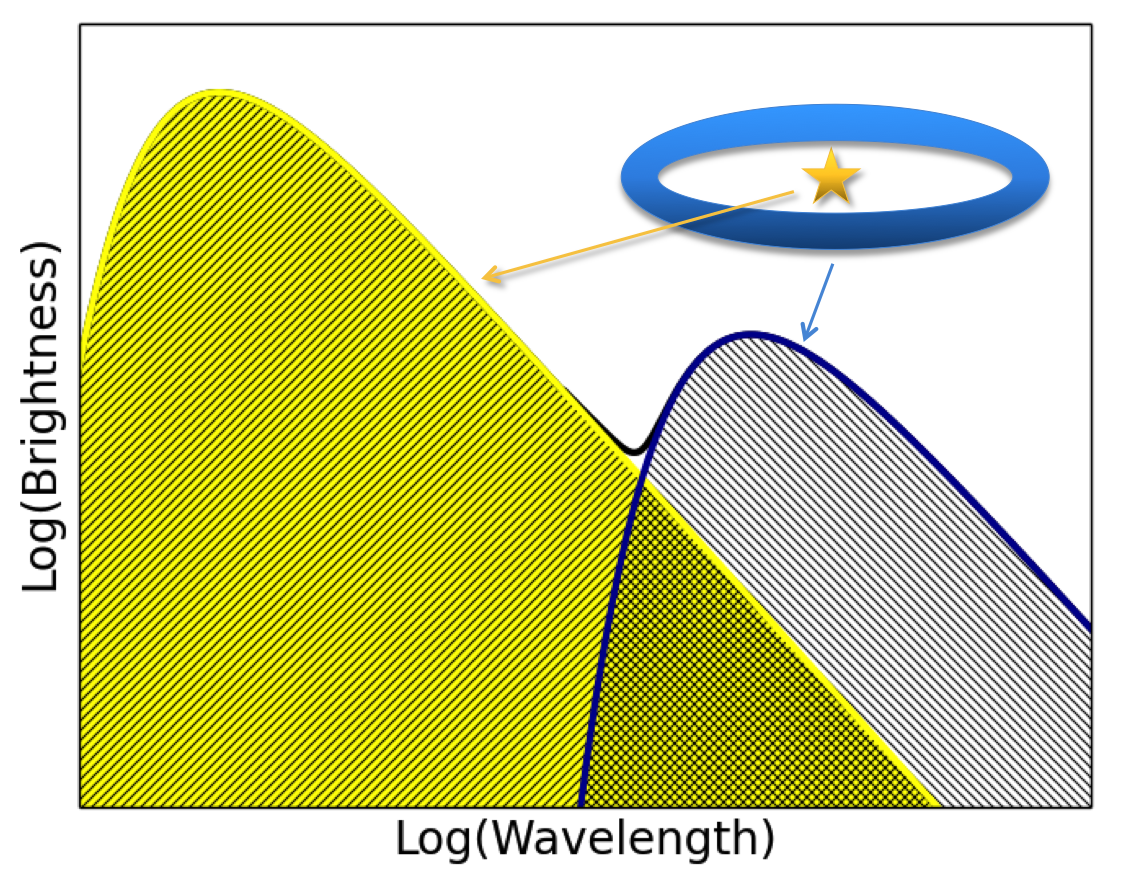
\includegraphics[width=0.7\textwidth]{49CET_SED_Cartoon_StarInsideDisk.png}
\caption{A representation of the SED of a star with a debris disk on a log-log plot. The star dominates at short wavelengths, whereas the disk emits the bulk of its radiation at longer wavelengths. Idea for cartoon courtesy of \cite{Stee14}.}
\label{fig:49CET_SED_Cartoon}
\end{figure}

These so-called ``debris disks" mark the final stage of disk evolution. They are characterized by optically thin dust emission and often do not exhibit any detectable gas emission. Because the lifetime of dust is generally on the order of tens of thousands of years \citep{Su13}, the grains in debris disks are assumed to be secondary, replenished through collisions of planetesimals. In order to excite rocky bodies to destructive collisional velocities, a stirring mechanism is needed. The gravitational influence of a planet can be responsible, but so-called ``self-stirring" is also possible, in which $\sim$ 1000\,km sized planetesimals coalesce before initiating a collisional cascade that results in small dust grains \citep{Keny04, Keny08, Must09, Moor13}. As a result of these stirring mechanisms, belts similar to the Solar System's asteroid and Kuiper belts are common in debris disks. 



These disks are usually identified by their fractional infrared excesses, $\sfrac{L_{IR}}{L_{bol}}$. \cite{Auma84} first noted this phenomena using the Infrared Astronomical Satellite (\textit{IRAS}), correctly attributing the excess to thermal emission of circumstellar grains heated by ultraviolet and visible light from the central star. As seen in Figure \ref{fig:49CET_SED_Cartoon}, the star dominates emission at short wavelengths, but the dust in the disk is brighter at longer wavelengths. Most searches for gas in debris disks have come up empty handed, supporting our assumption that gas and dust evolve simultaneously, but there are a handful of systems that break the norm. 
%relative contribution of small and large grains?

\section{Gas in Circumstellar Disks}

\subsection{Observing Gas in Disks}
In order to analyze the gas content of circumstellar material, observations look for both absorption and emission lines, with each able to reveal different aspects of the gas disk morphology. Temporally stable absorption lines with no velocity relative to the star give insight into the column density of the edge-on gas disk, whereas variable absorption and emission at a variety of relative velocities imply the presence of falling evaporating bodies \citep[FEBs,][]{Beus94} and help constrain the chemistry of the disk. In addition, resolved observations of the gas at millimeter wavelengths and complex modeling have revealed the size, scope, and properties of the gas disk. 

Hydrogen, despite being the dominant component of circumstellar disks, is difficult to observe. The ro-vibrational and rotational lines in the mid-IR are weak, and the strong electronic transitions emit in the ultraviolet where Earth's atmosphere is opaque \citep{Haba05}, though space-based observations are sensitive to these lines. Carbon monoxide (CO) is the most abundant molecule in circumstellar disks other than hydrogen, and it has strong rotational transitions at sub-millimeter and millimeter wavelengths, making it an ideal probe with which to analyze the gas content. Traces of other volatiles such as HCN, HCO+, CN, C$_{2}$H, NH$_{4}$, and polycyclic aromatic hydrocarbons (PAHs) have been detected in disks and help explore the gas disk chemistry \citep{Berg09}, but very low abundances make these observations taxing on telescope resources \citep{Viss11}.

\subsection{Gas-rich Debris Disks}

Using CO as the tracer, observations have shown that the bulk of primordial gas dissipates within $\sim$ 10\,Myr, with less than a Jupiter mass generally remaining after only a few Myr \citep{Zuck95}. This dispersal timescale lines up well with that for dust dispersal from protoplanetary systems, corroborating the view that gas and dust evolve together. However, the existence of gaseous debris disks, which display the secondary dust content of optically thin debris disks but retain enough molecular gas to be detectable at millimeter wavelengths, hints that other processes can shape the gas disk at later stages of disk evolution.  

Gas has been detected in edge-on debris disks with both far-UV \citep[$\beta$ Pic, $\sigma$ Her,][]{Robe00,Chen03} and optical spectra \citep[HD 32207, HD 172555,][]{Redf07,Kief14}. In $\beta$ Pic, stable absorption lines were detected in both CO and C\upperRomannumeral{1}, and a variable component was discovered in C\upperRomannumeral{1}. $\sigma$ Her shows signs of a radiatively driven wind that is blue-shifting gas liberated from collisions between parent bodies at $\sim$ 20\,AU. The optical photometry used by \citeauthor{Redf07} examined strong sodium lines to discover stable absorption by the gas in HD 32207, whereas \citeauthor{Kief14} inferred the presence of FEBs in HD 172555with variable Ca absorption lines. The proximity of $\beta$ Pic ($\sim$ 10\,pc) relative to these other systems has allowed its gas disk to be easily resolved by sub-millimeter observations \citep{Wiln11,Dent14}. Other than the disk around 20\,Myr old $\beta$ Pic, only a small selection of other gas-rich debris disks have been observed via emission spectroscopy of CO at millimeter wavelengths \citep[5\,Myr old HD 141569, 30\,Myr old HD 21997, 40\,Myr old 49 Ceti,][]{Wein00,Moor13,Kosp13, Zuck95}. Until this work, only HD 21997 has been resolved in both gas and dust emission at millimeter wavelengths, though the gas disk around 49 Ceti has been resolved in CO emission \citep{Hugh08}. These systems, taken together, provide a timeline to examine what processes are shaping the gas and dust as disks evolve, but each displays unique properties, indicating that this picture is not a simple one. 

49 Ceti sets the endpoint for describing the evolution of gas in debris disks, although it was not always known to be the oldest of these systems. For some time, it was thought to be 7.8\,Myr old based on evolutionary tracks that simultaneously considered accretion history \citep{Sies00,Thi01b}, but \cite{Rhee07} noted that 49 Ceti's galactic motions with respect to the Sun were not indicative of youth and suggested an age of 20\,Myr. With the classification of 49 Ceti as part of the Argus Association \citep{Zuck12}, this estimate was revised to its current best estimate of $\sim$ 40\,Myr, making it the oldest known main sequence star to contain a substantial reservoir of molecular gas. 

%The ages of these systems are significantly longer than the lifetimes of the constituent materials, so the fact that we see gas at all hints there might be secondary processes releasing gas in a small selection of systems. 

%\cite{Dent95} searched for 12CO around Vega, epsilon Eridanus, Fomalahut, beta leo, and beta pic with J2-1 and J3-2 on JCMT because J1-0 searches had come up empty handed... didn't find any CO emission. need higher sensitivity observations.  

%49 Ceti, an A star, provides a compelling research target, as it is one of only a handful of systems \citep[$\beta$ Pic, HD 21997, HD 141569, ][]{Dent14,Moor13,Kosp13,Wein00} that display the dust properties of optically thin debris disks but retain enough molecular gas to be detectable at millimeter wavelengths. 20 Myr old $\beta$ Pic, also an A star, displays an edge-on gaseous debris disk, and at only 19pc away, it has been studied extensively. Its disk has a dust mass of $\sim 8\times10^{-2}$ $M_{\rm Earth}$ and CO mass of $\sim 4\times10^{-5}$ $M_{\rm Earth}$ \citep{Dent14}. The micron-sized grains revealed in scattered light are essentially co-located with the millimeter grains seen by radio interferometers, with both grain populations peaking at 60\,AU from the star. This nearly matches the inner radius of the gas disk, which extends from 50 to 160 \,AU, peaking at 85 \,AU. Because the CO dissociation timescale is very short ($\sim$ 100 years) in $\beta$ Pic's strong interstellar radiation field, it is likely that the gas is being continually replenished in a ``birth ring" that is also responsible for producing the levels of dust that we see. 

%HD 21997 is a 30 Myr old A star that also hosts a gaseous debris disk. The dust disk extends from 55 to 150 \,AU and has a mass of $\sim 9\times10^{-2}$ $M_{\rm Earth}$ \citep{Moor13}, whereas an estimated $\sim 6\times10^{-2}$ $M_{\rm Earth} of CO extends from $\sim 25$ \,AU to  $\sim 140$ \,AU \citep{Kosp13}. Although the dust and gas disks overlap between 55 and 140 \,AU, within 55 \,AU there seems to be a dust-poor inner region. The distinct locations of the gas and dust hint that different processes may be shaping their morphologies. In fact, \citeauthor{Kosp13} suggest the gas is primordial, but \citeauthor{Moor13} hint that the dust is secondary. 

%HD 141569, an A star $\sim$ 110pc away that is 5Myr old, displays CO emission in addition to displaying the qualities of a debris disk. Scattered light imaging by \cite{Wein00} reveals that the disk extends out to $\sim$ 360\,AU with a gap in the disk at $\sim$ 250\,AU. Gaps like these are suggestive of continual clearing and secondary dust production processes. \cite{Brit07} find that the gas emission comes from within $\sim$ 40\,AU of the star, but it is unclear if the dust traces the gas, as the scattered light imaging is only able to see micron-sized grains at greater than $\sim$ 70\,AU and millimeter observations have not been performed. 

\section{49 Ceti's Gaseous Debris Disk}
\subsection{49 Ceti's Dust Disk}
49 Ceti was first noted as a disk-hosting candidate by \citet*{Sada86}, who correlated objects in the Yale Bright Star Catalog with those that displayed significant 60\,$\mu m$ excesses with \textit{IRAS}. \cite{Jura93} went one step further, showing that 49 Ceti, along with $\beta$ Pic and HR 4796, had $\sfrac{F_{60\,\mu m}}{F_{V}} < 0.1$, implying $\tau~<~10^{-3}$ and thus an optically-thin dust disk. 

%This study will give us a look into whether the gas and dust are dispersing simultaneously and whether the gas is primordial or second generation (created from the collisions of comets), both of which have implications for the timeframe during which giant gas planets can form. 


%Protoplanetary disks, a natural consequence of stellar formation, are planetary nurseries with their huge

%This transitional period is distinguished by an inside-out clearing of sub-mm dust from the star and dispersal of gas from the system which is first identified by a lack of near-IR emission due to the dearth of hot dust close to the star. Photoevaporation by high-energy photons and gravitational clearing by massive planets are the primary mechanisms that disperse the inner dust and gas \citep{Wyat14}. However, transition disks are rare in the stellar neighborhood, as there are few pre-main sequence stars within $\sim$ 100pc. This makes resolved observations, which are needed to confirm the disk morphology, difficult to come by. 

%Understanding this liminal stage is crucial for understanding planet formation. 


%(Something about protoplanetary, debris disks, optical depth differences? see Wyatt 03?)

The spatial distribution of dust was first investigated with Keck imaging at 17.9$\,\mu m$, which revealed low-level emission extending 1.5$''$ (100\,AU) at a position angle of 40$^{\circ}$ \citep{Guil99}, though these data are unpublished. Simultaneous modeling of the mid-IR image and \textit{IRAS} fluxes hinted at a two part disk structure composed of a warm inner component and cold dense outer component. Keck N-band (10$\,\mu m$) images by \cite{Jaya01} marginally resolved extended structure consistent with \citeauthor{Guil99}, but the first sub-arcsecond resolution images of 49 Ceti's disk came from significantly longer exposures with Keck \citep{Wahh07}. These images, at 12.5 and 17.9$\,\mu m$, showed that the disk extended along a NW-SE axis with an inclination of 60$^{\circ} \pm 15^{\circ}$. An optically thin dust disk model with one characteristic grain size was unable to recreate the spatially resolved data and fluxes from the literature, but a model with small grains (a $\sim$ 0.1\,$\mu m$) between 30\,AU and 60\,AU from the star and an extended disk of larger grains (a $\sim$ 15\,$\mu m$) was a good fit. In this model, the undetected outer disk, which contained the majority of the dust mass, was necessitated by the fit to the fluxes at far-IR wavelengths.

Longer wavelength observations of 49 Ceti with Herschel show IR excesses at 70, 160, 260, 350, and 500$\,\mu m$ and resolved extended structure along the major axis at 70$\,\mu m$ \citep{Robe13}. The deconvolved image, with a HWHM of 3.4 arcsec along the major axis, suggests that the semi-major axis of the disk is $\sim$ 200\,AU and shows no signs suggestive of a central clearing or any large-scale asymmetry. 

Attempts to observed the disk in scattered light with the Near-Infrared Camera and Multi-Object Spectrometer (NICMOS) aboard Hubble did not detect any scattered light emission beyond an angular separation of 1.6 arcsec from the central star \citep{Wein99}. This discrepancy will be explored in Section \ref{MidIR}. %Derived fluxes at millimeter wavelengths have thus far been inconsistent with either a thermal spectrum ($F_{\lambda} \propto \lambda^{-2}}$) or optically thin dusty disk spectrum at long wavelengths ($F_{\lambda} \propto \lambda^{-3}}$). \cite{Song04} report a JCMT/SCUBA 850 $\mu m$ flux of 8.2 $\pm$ 1.9mJy, while \cite{Bock94} measured an IRAM 1200$\mu m$ flux of 12.7 $\pm$ 2.3 mJy. Higher signal-to-noise observations at 850 and 1200$\mu m$ will be presented in this work, ironing out this kink in the long-wavelength regime. 

%(a $\sim$ 1$\mu$m) between 30\,AU and 60\,AU from the star are responsible for the majority of mid-infrared excess, whereas an extended disk of larger grains (a $\sim$ 15$\mu$m) is responsible for the rest of the infrared excess. 

\subsection{49 Ceti's Gas Disk}

The molecular gas content of 49 Ceti's disk has been both detected with single radio dishes and resolved with interferometric observations. \cite{Zuck95} marginally detected the CO J=2-1 line with IRAM, showing 49 Ceti contained a measurable amount of gas. JCMT observations of the CO J=3-2 line set an upper limit on the CO mass of 0.02\,M$_{\oplus}$ \citep{Coul98}, which suggests no more than $\sim$ 200\,M$_{\oplus}$ of H$_{2}$. Hydrogen was observed directly in its lowest rotational transition with SWS/ISO, suggesting a lower limit of 110\,M$_{\oplus}$ \citep{Thi01a}, but \cite{Chen06} and \cite{Carm07} did not confirm this detection with \textit{Spitzer}/IRS and VLT/CRIRES, respectively. Modeling by \cite{Dent05} of updated JCMT CO J=3-2 observations suggested a compact disk inclined at $\sim$ 16$^{\circ}$ or a larger ring ($\sim$ 50\,AU) inclined at 35$^{\circ}$, though the secondary model was unable to recreate the high-velocity wings apparent in the line profile. The first resolved images of the gas disk at arcsecond resolution were obtained using the Sub-Millimeter Array (SMA) by \cite{Hugh08}, showing CO J=2-1 emission around 49 Ceti in Keplerian rotation between 40 and 200\,AU, including a central clearing, potentially consistent with photoevaporation.

\section{49 Ceti's Implications for the Evolution of Circumstellar Material}

49 Ceti's debris disk has never been imaged at millimeter wavelengths, and observations in this regime provide an important tracer of the large grains in disks that probe the distribution and dynamics of parent planetesimals. In addition, previous examinations of the gas disk were performed at low resolution with low signal-to-noise, whereas higher sensitivity observations can reveal subtle details about the gas morphology. In this thesis, we present new observations from the Combined Array for Research in Millimeter-wave Astronomy (CARMA) and the Atacama Large Millimeter Array (ALMA) that resolve the extended dust disk at sub-arcsecond resolution for the first time (the gas analysis will be described elsewhere). The level of detail now available in constraining the location, mass, and dynamics of planet forming material with these observations gives us fresh insight into the mechanics that shape circumstellar disks at this late stage of disk evolution. In consideration with other systems, we are helping to complete the picture of how and why gas and dust disperse, which has important implications for the timescale of giant planet formation. Ultimately, making sense of the processes that shape these disks are essential for understanding how solar systems such as our own formed, and will help us figure out how ordinary or rare our Solar System really is. 

%Unraveling these mysteries requires a careful consideration of all pieces of evidence, and our analysis of 49 Ceti is helping us connect the dots to see the big picture.


%which in turn (has implications for) how 

%These systems, taken together, provide somewhat of a timeline to examine what processes are shaping the gas and dust as disks evolve, but each display unique properties, indicating that this picture is in no way a simple one. 

%gives us insight into whether the dust and gas is primordial or secondary. In addition, analysis in combination with younger gaseous debris disks will give us insight into the timescale for giant planet formation. 

%\ifthenelse{\isodd{\thepage}}{\clearemptydoublepage}{}
